\chapter{Experimental Setting}

The current chapter is divided into two sections. In the first one the benchmark of the experiment will be described. In the second one the same experiment applied to humans and its results will be discussed.

\section{Benchmark}

\subsection{Test Functions}

The experiment described in this work is about maximize black-box functions adopting an RL based approach. The first important choice is about selecting suitable \textit{test functions}. In applied mathematics, test functions, also known as \textit{artificial landscapes}, are useful to evaluate characteristics of optimization algorithms. Four test functions have been chosen for this work:

\begin{itemize}
	\item Himmelblau' s Function;
	\item Sphere Function;
	\item Beale Function;
	\item Styblinski-Tang' s Revised Function.	
\end{itemize}

\subparagraph{Himmelblau' s Function} In mathematical optimization, Himmelblau' s function is a continuous, bivariate, multi-modal function. The original function is defined by: 

\begin{equation}
	f(x, y) = (x^2 + y -11)^2 + (x + y^2 - 7)^2
\end{equation}

It has four local minima :

\begin{itemize}
	\item $f(3.0, 2.0) = 0.0$;
	\item $f(-2.805118, 3.131312) = 0.0$;
	\item $f(-3.779310, -3.283186) = 0.0$;
	\item $f(3.584428, -1848126) = 0.0$.
\end{itemize}
	
The function can be defined on any input domain but it is usually evaluated on $x \in [-5, 5]$ and $y \in [-5, 5]$.

\begin{figure}[h!]
	\centering
	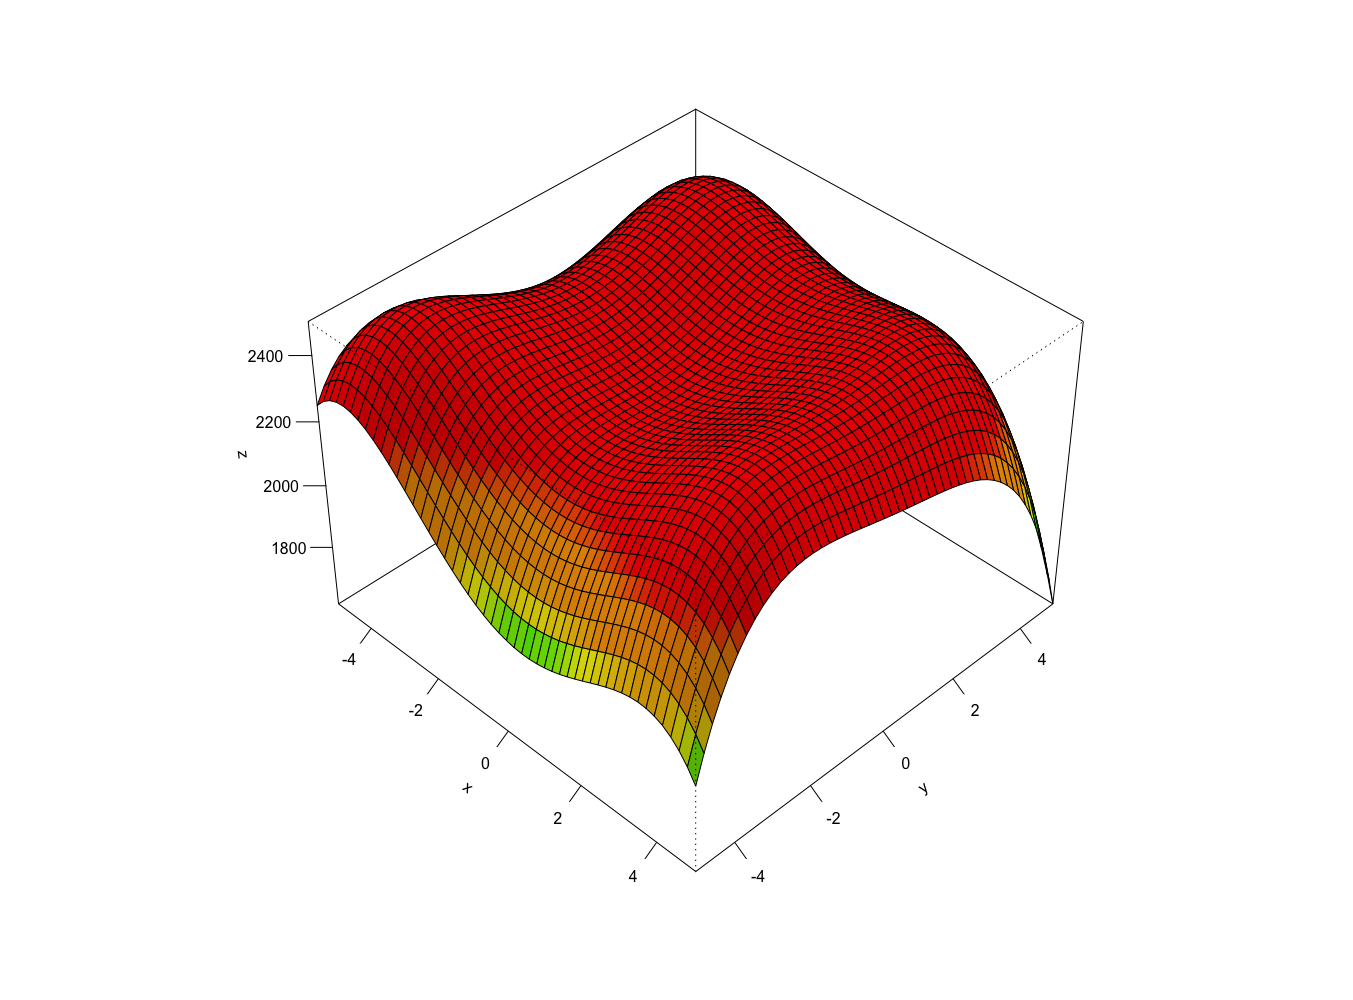
\includegraphics[width= 12cm, height = 12cm]{modifiedHimmelblau.png}
	\caption{Customized Himmelblau' s Function.}
	\label{fig:CustomizedHimmelblauFunction}
\end{figure}

Because of the aim to maximize the function has been inverted as follow :

\begin{equation}
f(x, y) = -(x^2 + y -11)^2 + (x + y^2 - 7)^2
\end{equation}

it has been picked up of $2500$ units in order to have as less as possible negative values. So the final adopted function is :
 
\begin{equation}
f(x, y) = -(x^2 + y -11)^2 + (x + y^2 - 7)^2 + 2500
\end{equation}

This function has its global maximum in $f(x, y) = 2500$. 

In order to represent this customized version of Himmelblau' s Function using Java Graphical Environment, it has been mapped in a space of $600 \times 600$ pixels and it has been properly rotated. The resulting contour plot is the one represented in figure ~\ref{fig:ContourPlotCustomizedHimmelblauFunction}. \\

\begin{figure}[h!]
	\centering
	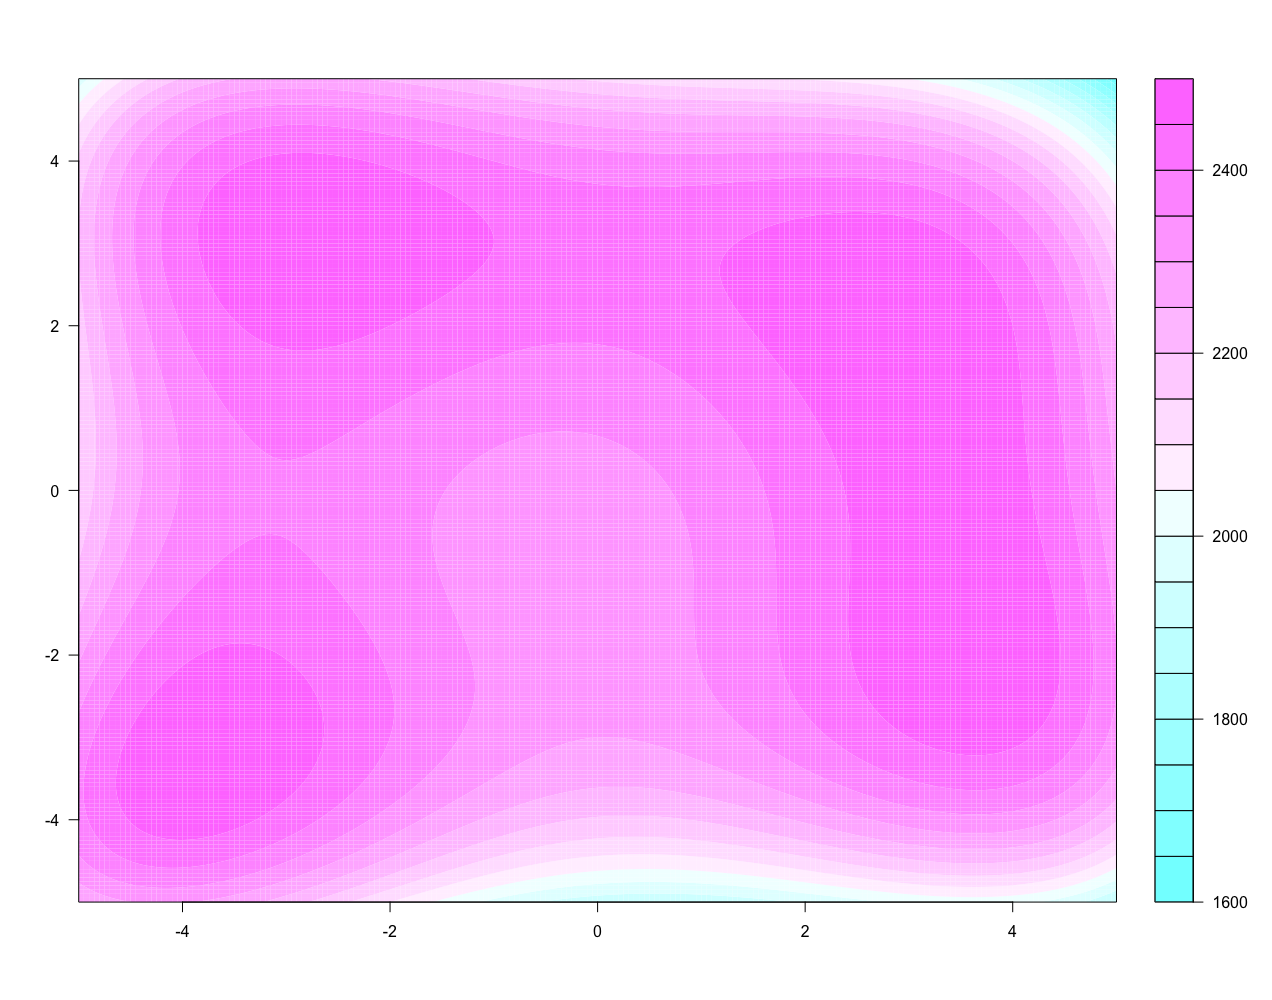
\includegraphics[width= 7cm, height = 7cm]{himmelblau.png}
	\caption{Contour plot of customized version of Himmelblau' s Function.}
	\label{fig:ContourPlotCustomizedHimmelblauFunction}
\end{figure}
 
\subparagraph{Sphere Function} In mathematical optimization, Sphere function is a continuous, bivariate, multi-modal function. \\

The original function is defined by: 

\begin{equation}
f(x, y) = (x^2 + y^2) 
\end{equation}

It has a global minimum in $f(x, y) = 0$.

The function can be defined on any input domain but it is usually evaluated on $x \in [-10, 10]$ and $y \in [-10, 10]$. 

\begin{figure}[h!]
	\centering
	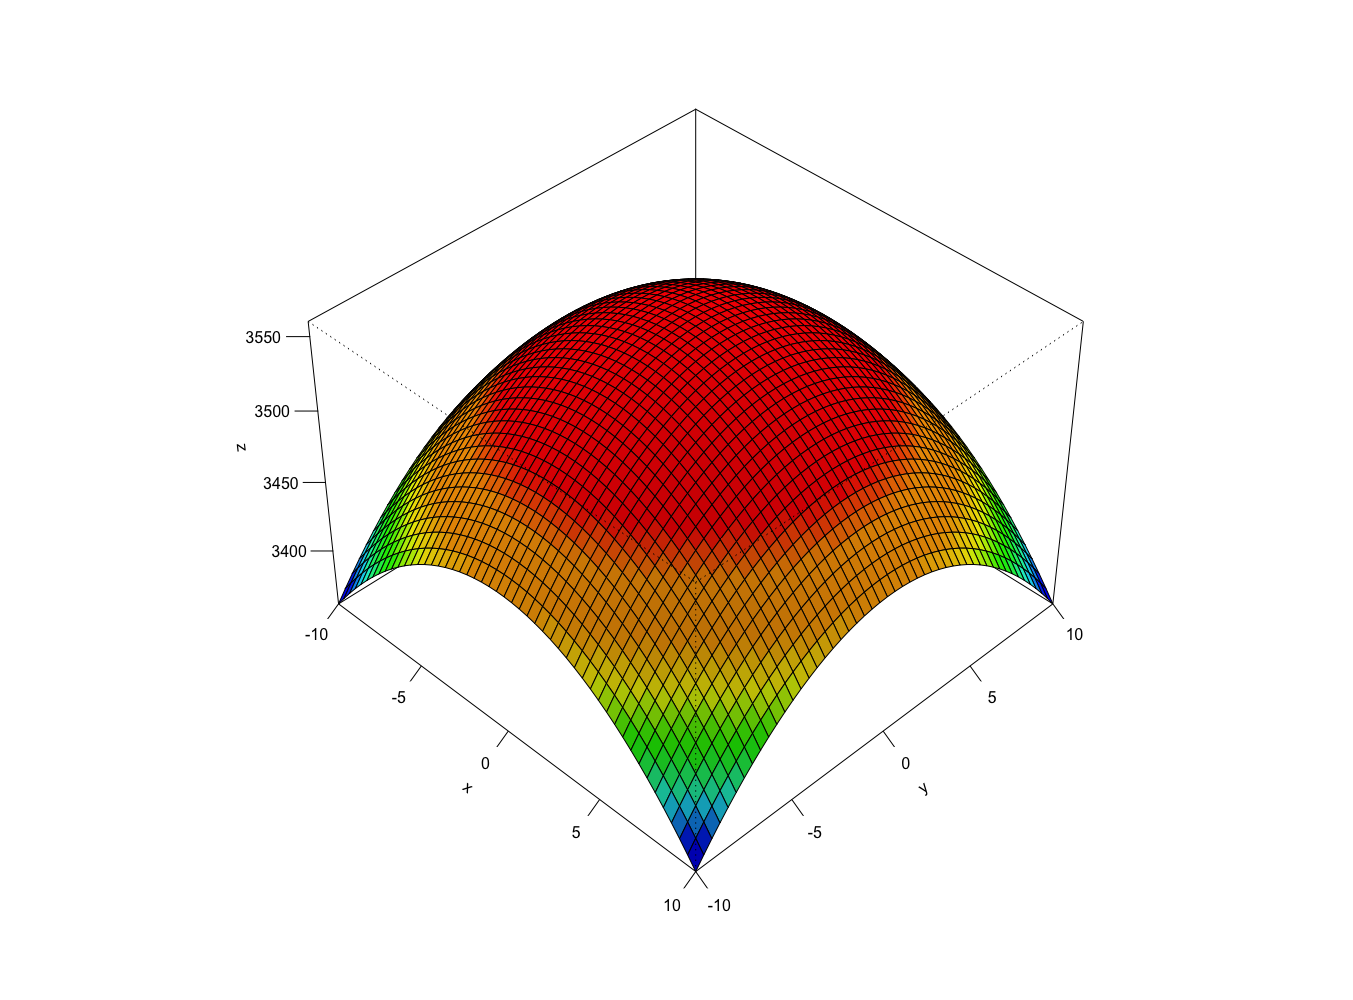
\includegraphics[width= 12cm, height = 12cm]{customizedParaboloid.png}
	\caption{Customized Paraboloid of Revolution.}
	\label{fig:CustomizedParaboloidOfRevolution}
\end{figure}

Because of the aim to maximize, the function has been inverted as follow :

\begin{equation}
f(x, y) = -(x^2 + y^2)
\end{equation}

and it has been picked up of $3560$ units in order to have as less as possible negative values. So the final adopted function is :

\begin{equation}
f(x, y) = -(x^2 + y^2) + 3560
\end{equation}

This function has its local maximum in $f(x, y) = 3560$.

In order to represent this customized version of Sphere function function using Java Graphical Environment, it has been mapped in a space of $600 \times 600$ pixels and it has been properly rotated. The resulting contour plot is the one represented in figure ~\ref{fig:ContourPlotCustomizedParabolicFunction} 

\begin{figure}[h!]
	\centering
	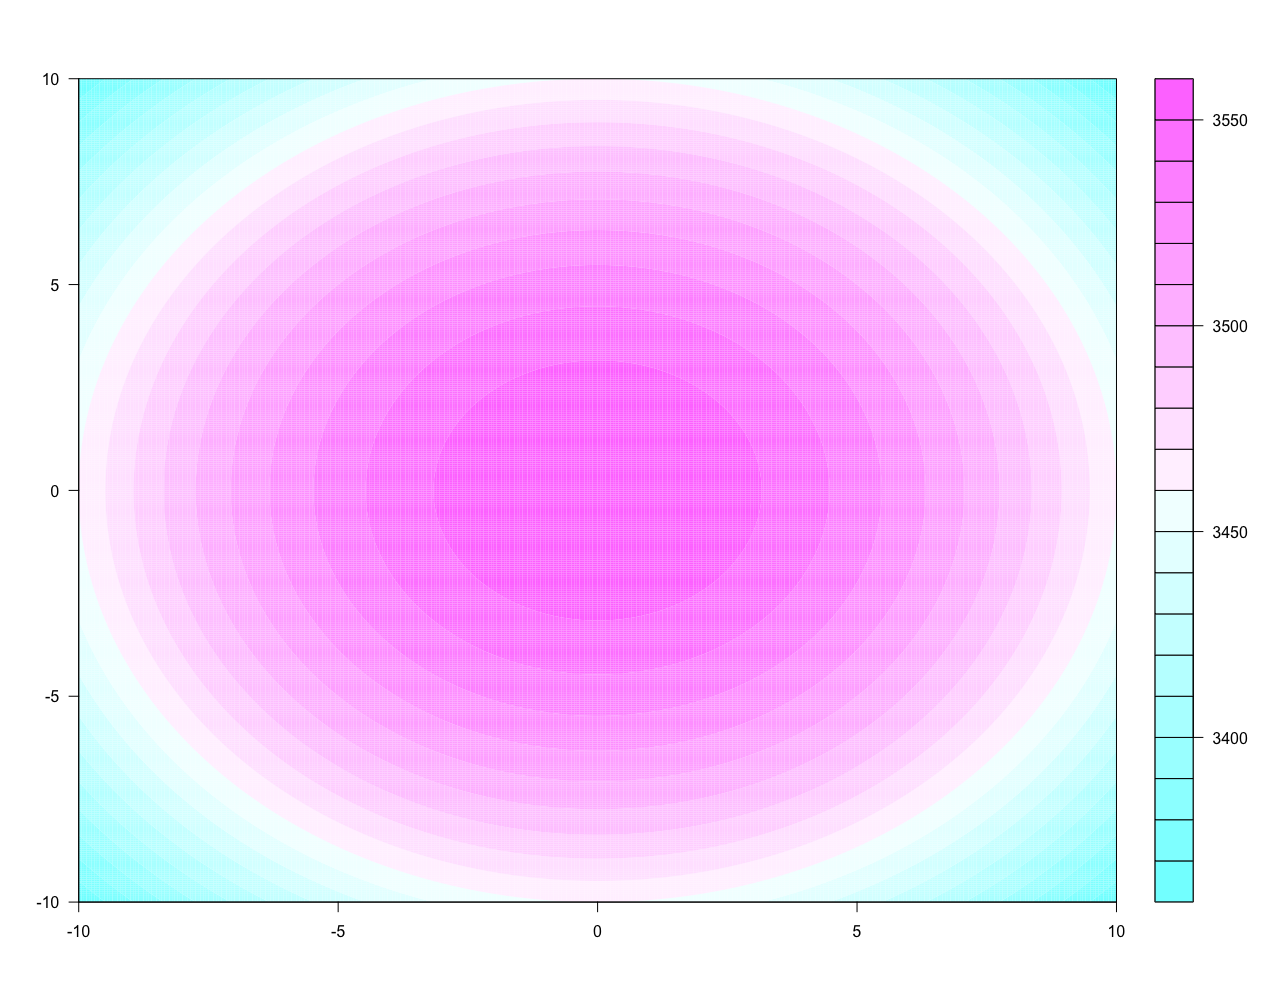
\includegraphics[width= 7cm, height = 7cm]{parabolic.png}
	\caption{Contour plot of customized Parabolic Function.}
	\label{fig:ContourPlotCustomizedParabolicFunction}
\end{figure}

\subparagraph{Beale Function} In mathematical optimization, Beale Function is a continuous, multi-modal function defined on a multi-dimensional space. The function is defined by: 

\begin{equation}
f(x, y) = (1.5 - x + xy)^2 + (2.25 - x + xy^2)^2 + (2.625 - x + xy^3)^2
\end{equation}

The function can be defined on any input domain but it is usually evaluated on $x \in [-3, 3]$ and $y \in [-3, 3]$. \\

It has one global minimum in: $f(x, y) = 0$. 

Because of the aim to maximize, it has been inverted as follow:

\begin{equation}
f(x, y) = -((1.5 - x + xy)^2 + (2.25 - x + xy^2)^2 + (2.625 - x + xy^3)^2)
\end{equation}

\begin{figure}[h!]
	\centering
	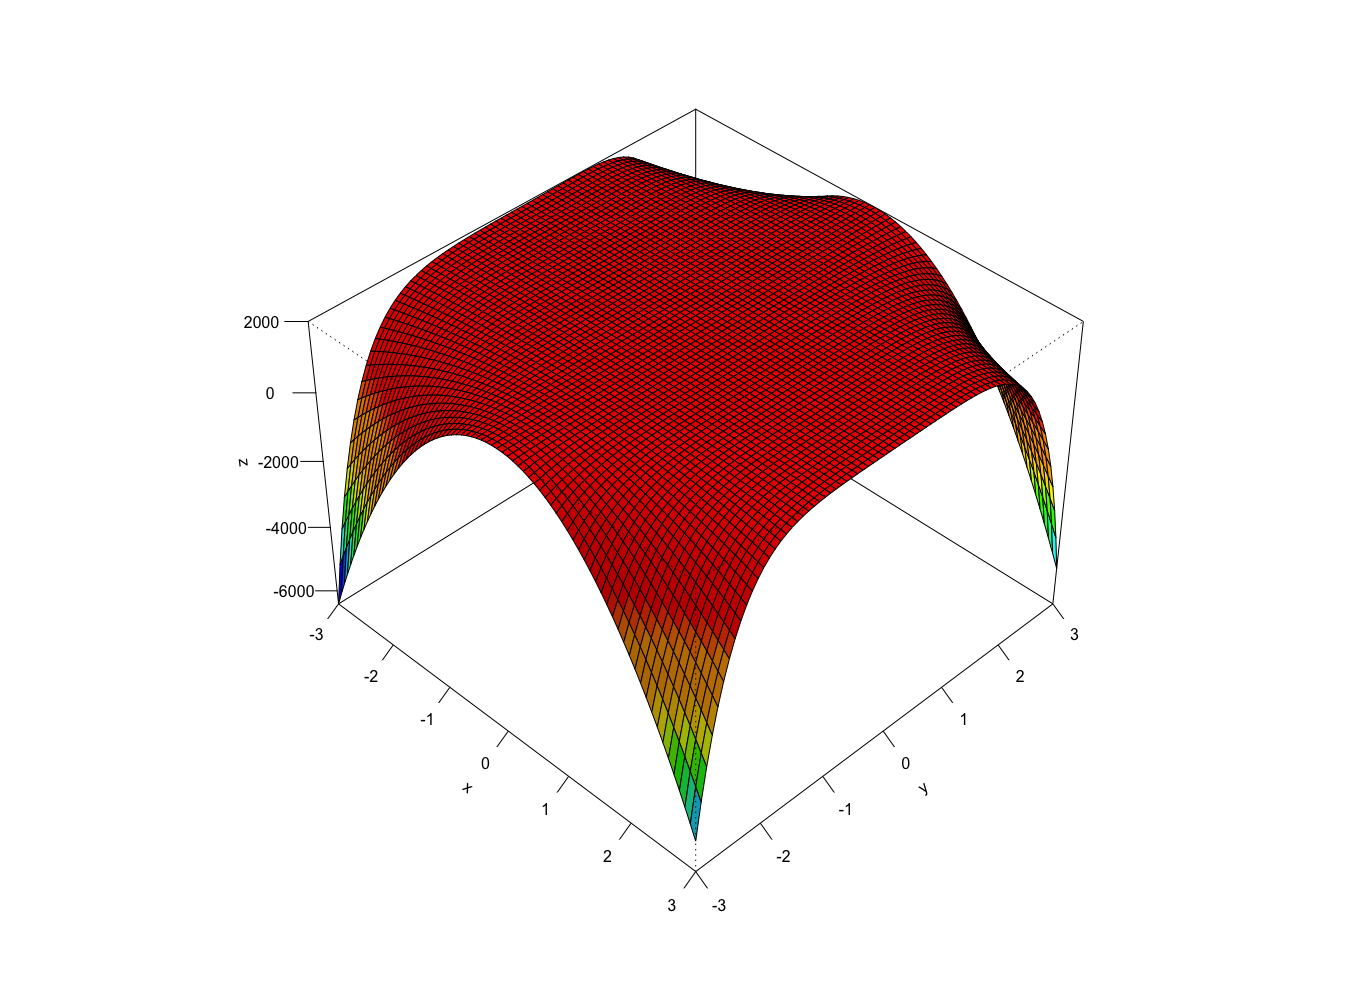
\includegraphics[width= 12cm, height = 12cm]{customizedBeale.png}
	\caption{Customized Beale Function.}
	\label{fig:CustomizedBealeFunction}
\end{figure}

and it has been picked up of $2000$ units in order to have as less as possible negative values. So the final adopted function is :

\begin{equation}
f(x, y) = -((1.5 - x + xy)^2 + (2.25 - x + xy^2)^2 + (2.625 - x + xy^3)^2) + 2000
\end{equation}

This customized function has its global maximum in $f(x, y) = 2000$. \\

In order to represent this function using Java Graphical Environment it has been mapped in a space of $600 \times 600$ pixels and it has been properly rotated. The resulting contour plot is the one represented in figure ~\ref{fig:ContourPlotCustomizedBealeFunction} 

\begin{figure}[h!]
	\centering
	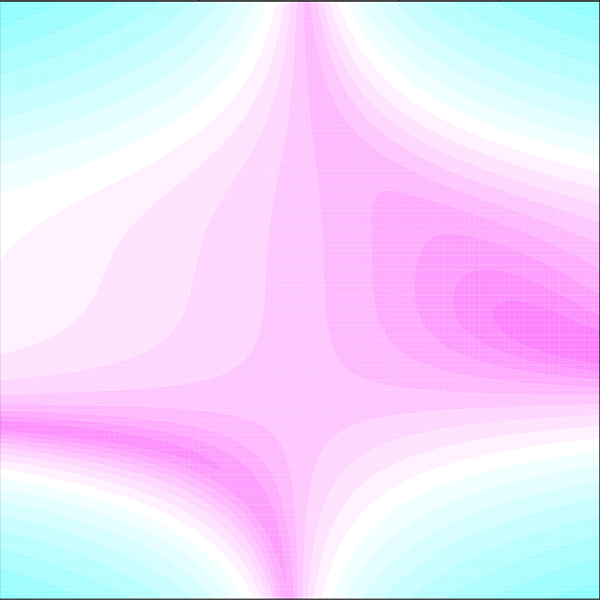
\includegraphics[width= 7cm, height = 7cm]{beale.png}
	\caption{Contour plot of customized Beale Function.}
	\label{fig:ContourPlotCustomizedBealeFunction}
\end{figure}

\subparagraph{Styblinski-Tang Revised Function} In mathematical optimization, Styblinski-Tang Function is a continuous, multi-modal function defined on a multi-dimensional space. The original function is defined by :

\begin{equation}
	f(x) = \dfrac{\sum_{i=1}^{n} x_{i}^4 -16x_{i}^2 +5x_{i}}{2}
\end{equation}

\begin{figure}[h!]
	\centering
	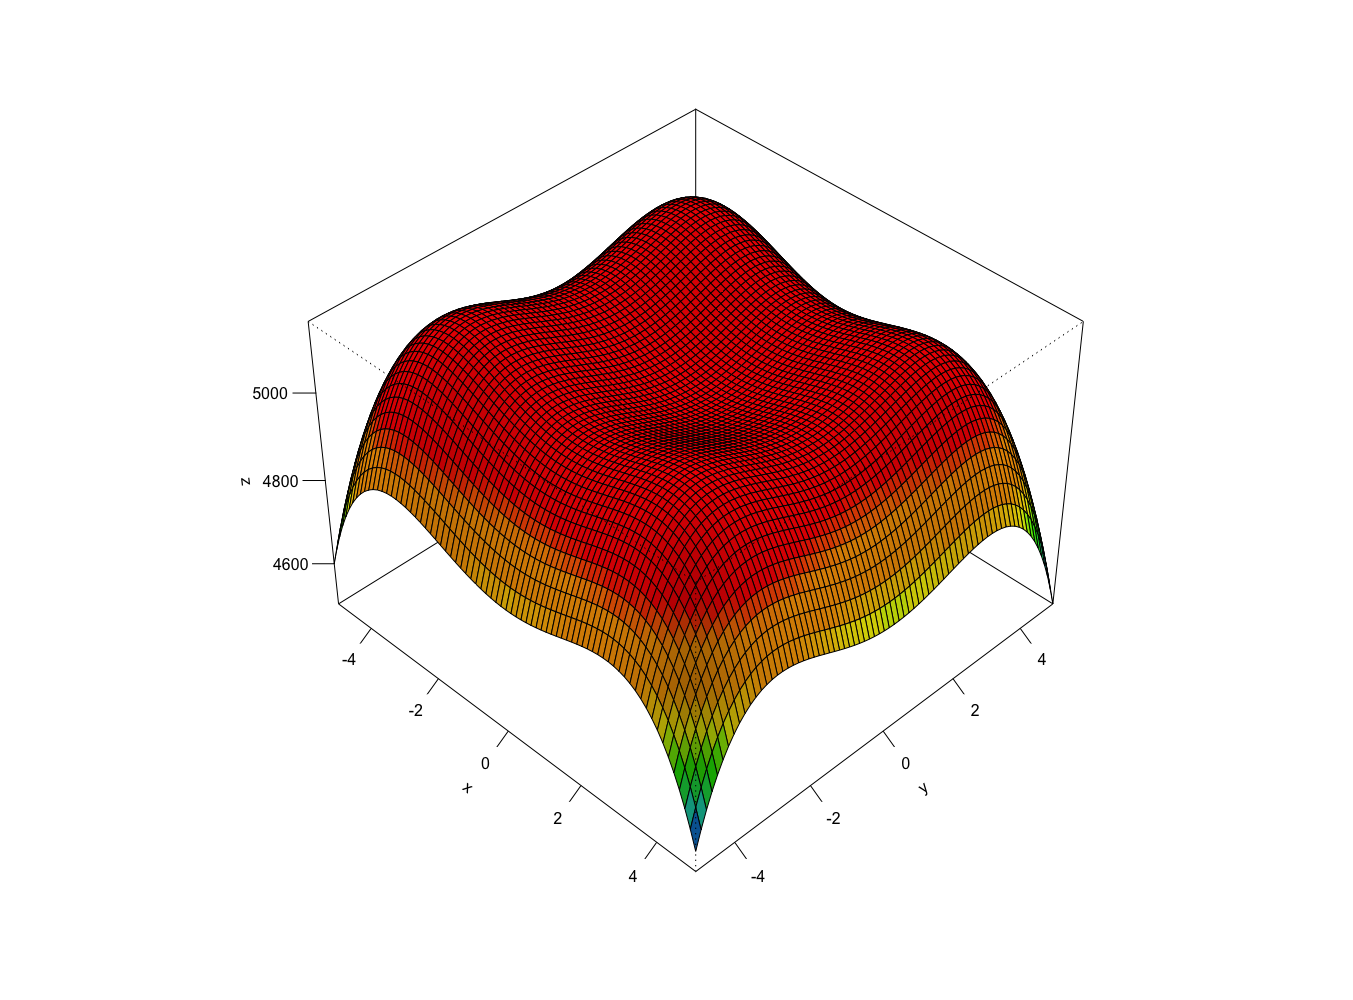
\includegraphics[width= 12cm, height = 12cm]{customizedStyblinski.png}
	\caption{Customized Styblinski Function.}
	\label{fig:CustomizedStyblinskiFunction}
\end{figure}

In this thesis the bivariate version of the original function multiplied by two in order to make it less flatten, is considered:

\begin{equation}
f(x, y) = (x^4 - 16x^2 + 5x) + (y^4 - 16y^2 + 5y).
\end{equation}

The function can be defined on any input domain but it is usually evaluated on $x \in [-5, 5]$ and $y \in [-5, 5]$. \\

Because of the aim to maximize, it has been inverted as follow :

\begin{equation}
f(x, y) = -((x^4 - 16 * x^2 + 5 * x) + (y^4 - 16 * y^2 + 5 * y))
\end{equation}

and it has been picked up of $5000$ units in order to have as less as possible negative values. So the final adopted function is: 

\begin{equation}
f(x, y) = -((x^4 - 16 * x^2 + 5 * x) + (y^4 - 16 * y^2 + 5 * y)) + 5000
\end{equation}

This customized function has its global maximum in $f(x, y) = 5156.6638$. In order to represent this function using Java Graphical Environment it has been mapped in a space of $600 \times 600$ pixels and it has been properly rotated. The resulting contour plot is the one represented in figure ~\ref{fig:ContourStyblinskiFunction}.

\begin{figure}[h!]
	\centering
	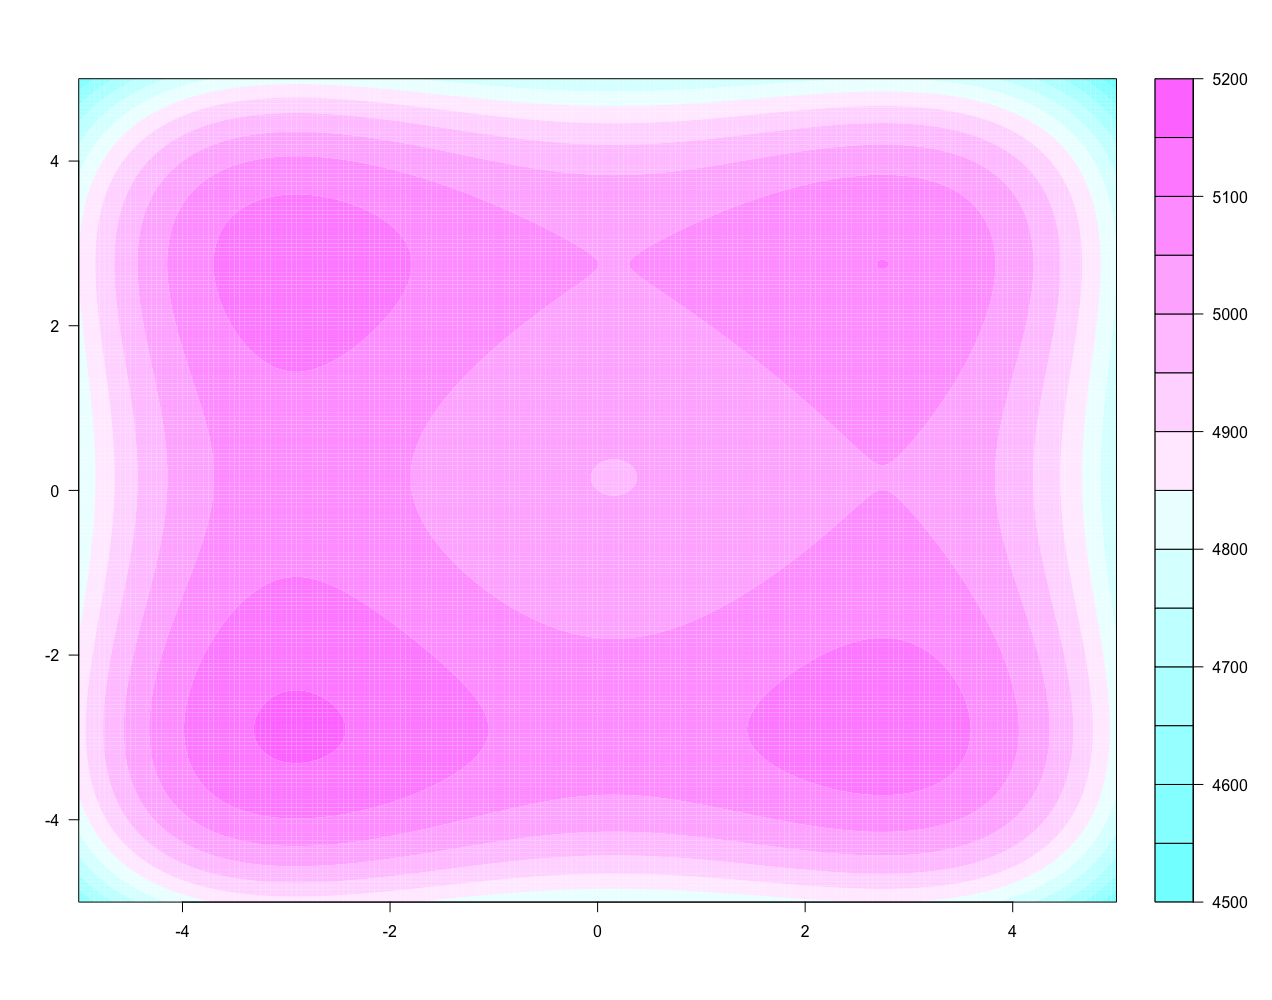
\includegraphics[width= 7cm, height = 7cm]{styblinski.png}
	\caption{Contour plot of customized Styblinski Function.}
	\label{fig:ContourStyblinskiFunction}
\end{figure}

\begin{sidewaystable} 
	\centering
	\caption{Objective Functions'  Summary Table}
	\begin{tabular}
		{l l l l l} \hline Name & Formula & Domain & Optimal \textit{f} & Sketch \\
		\hline Himmelblau & \vtop{\hbox{\strut $f(x, y) = - ((x^2 + y -11)^2+$}\hbox{\strut $+(x + y^2 - 7)^2) + 2500$}} & $x, y \in [-5;+5]$ & $2500$ & \parbox[c]{1em}{
			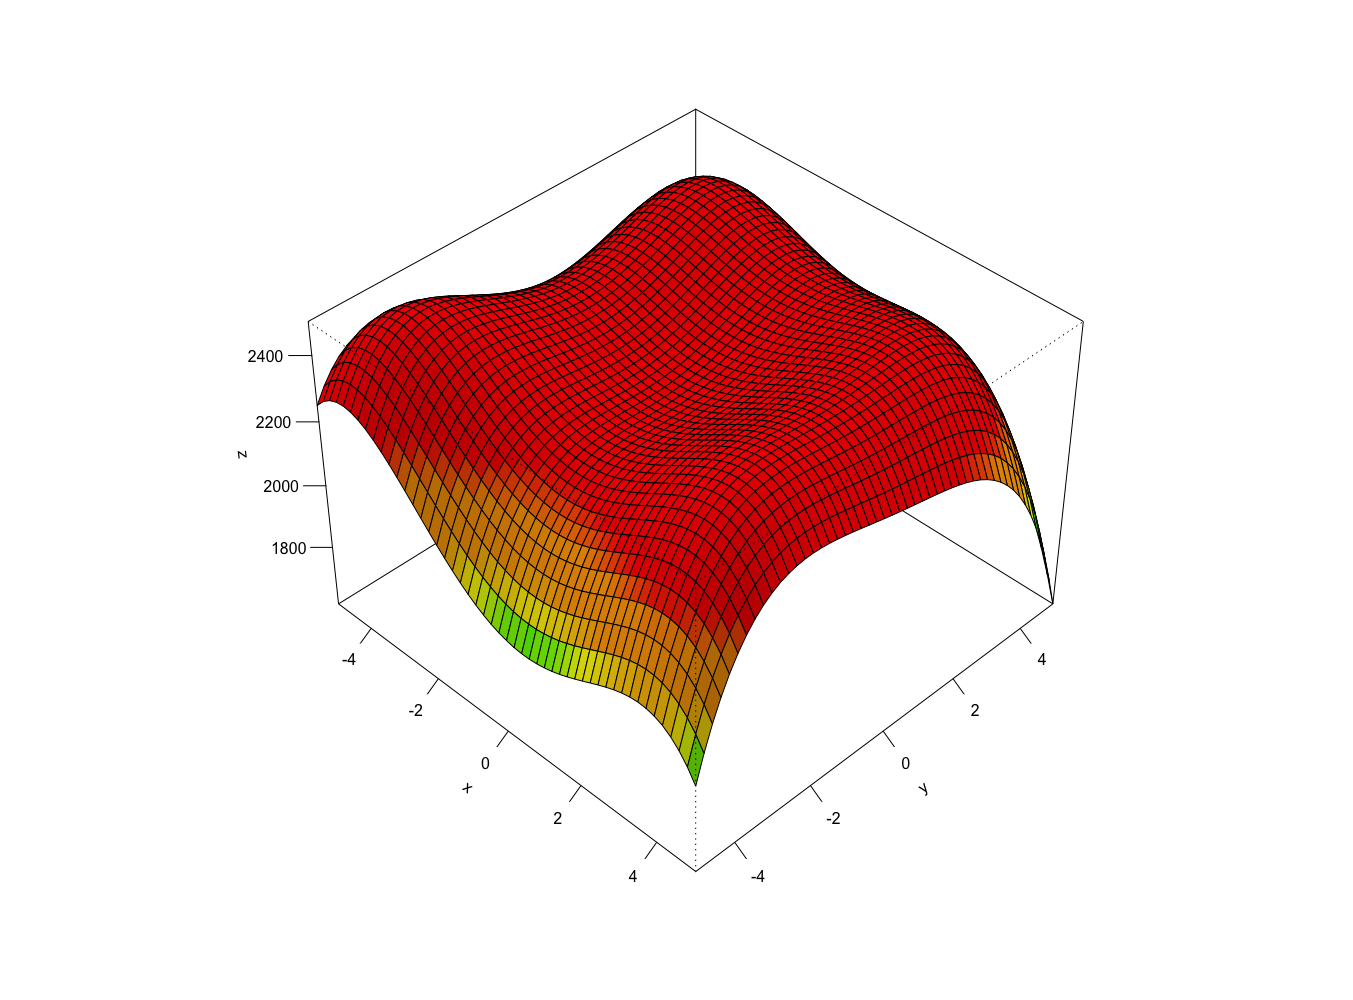
\includegraphics[width=1.7in]{modifiedHimmelblau}} \\
		Sphere & $f(x, y) = -(x^2 + y^2) + 3560$ &$x, y \in [-10;+10]$ & $3560$ & \parbox[c]{1em}{
			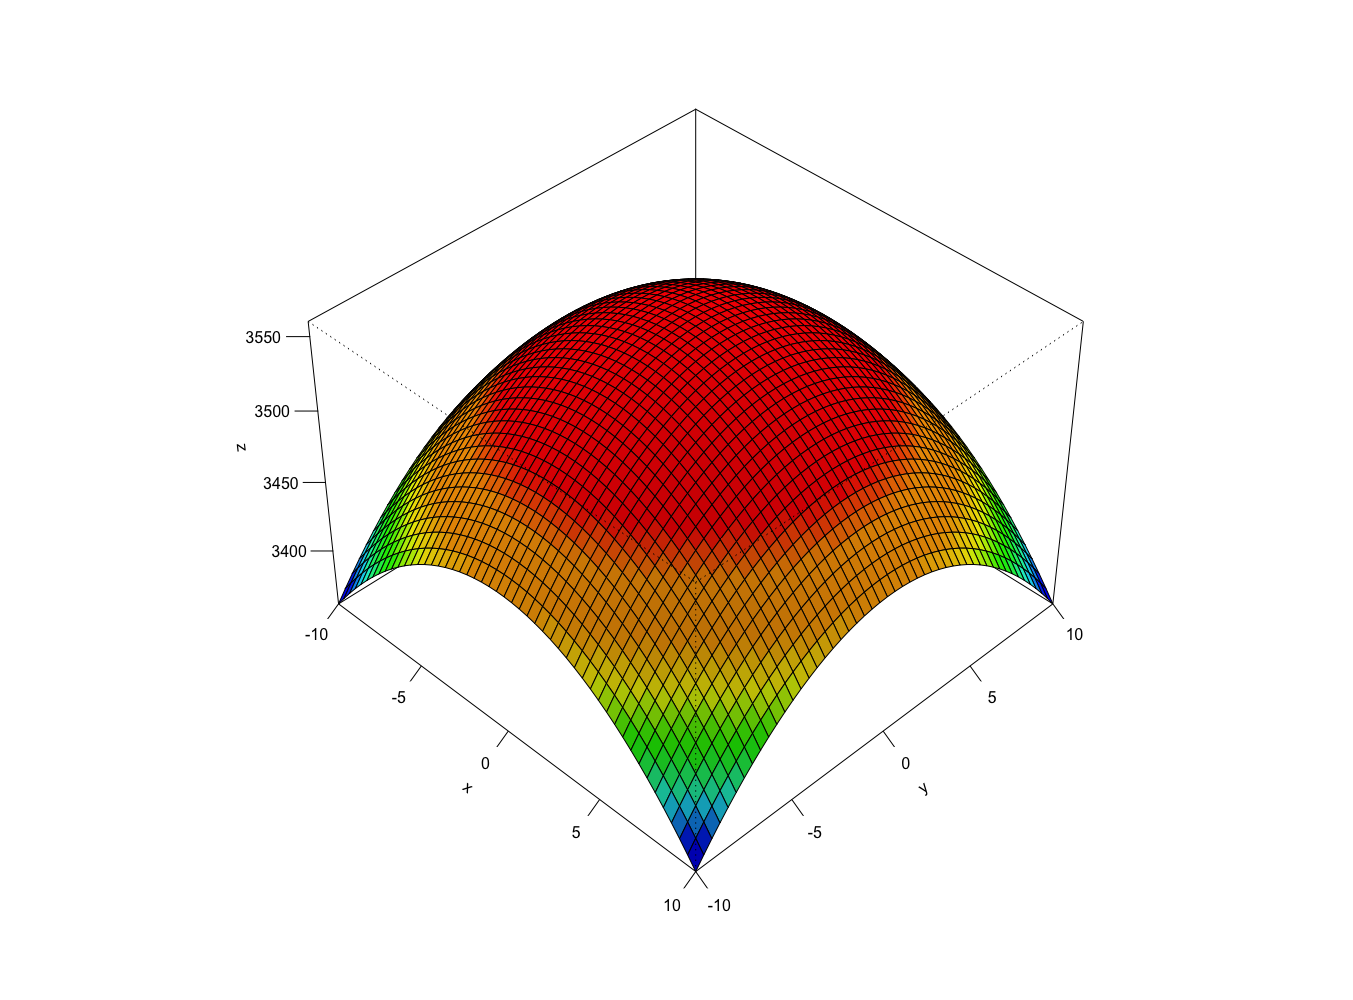
\includegraphics[width=1.7in]{customizedParaboloid}} \\
		Beale & \vtop{\hbox{\strut $f(x, y) = - ((1.5 - x + xy)^2 + ) $}\hbox{\strut $+ (2.25-x+xy^2)^2 + $}\hbox{\strut $+ (2.625 -x+xy^3)^2) + 2000 $}} &$x, y \in [-3;3]$ & $1000$ & \parbox[c]{1em}{
			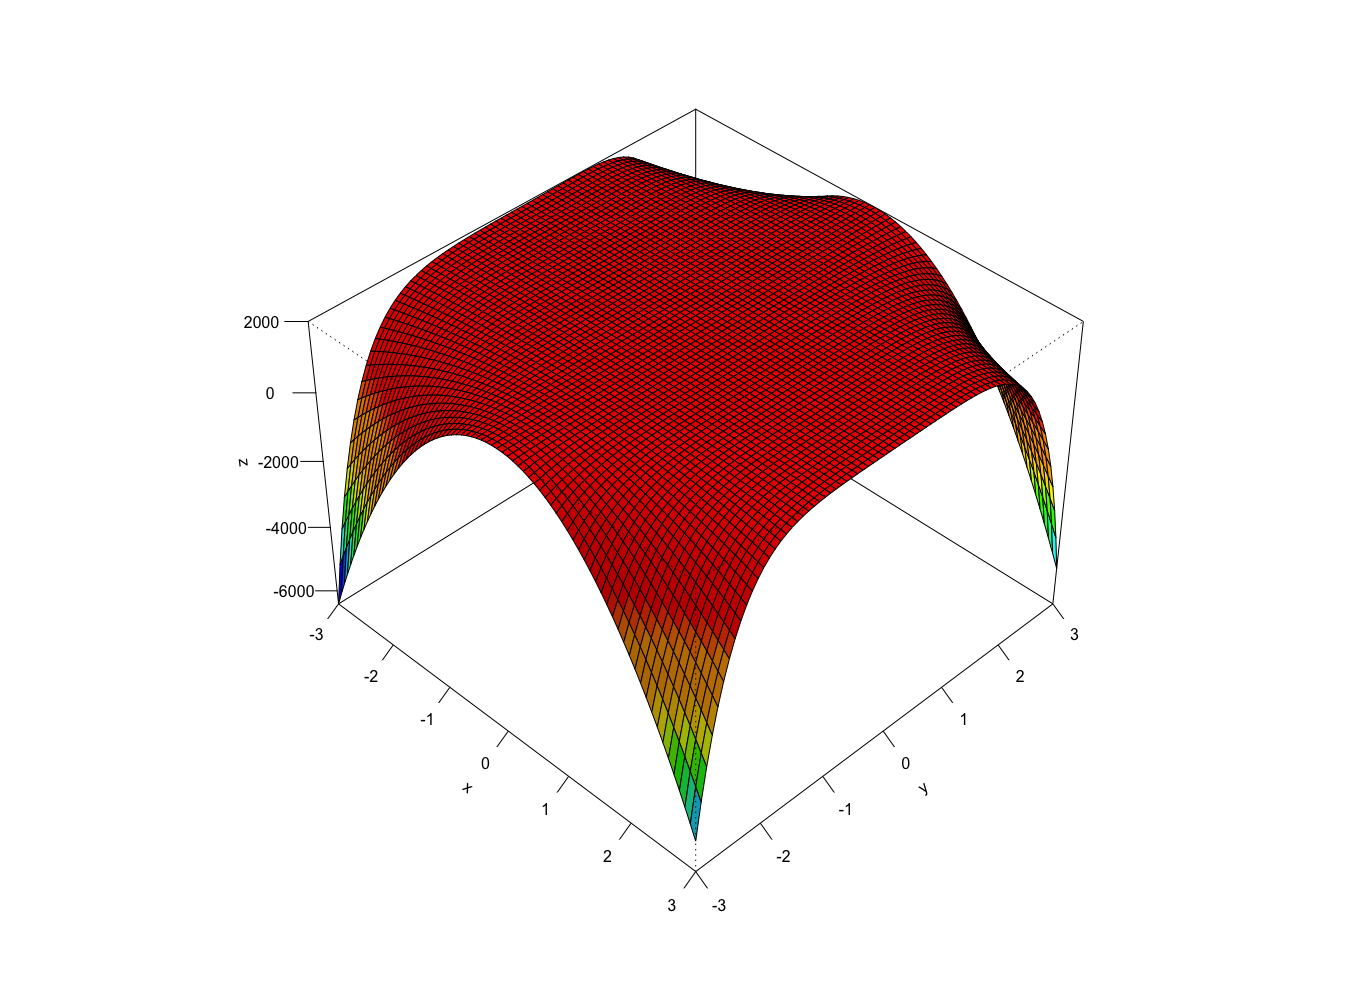
\includegraphics[width=1.7in]{customizedBeale}} \\
		Styblinski-Tang & \vtop{\hbox{\strut $f(x, y) = -((x^4 - 16 * x^2 + 5 * x) + $}\hbox{\strut $(y^4 - 16 * y^2 + 5 * y)) + 5000$}} &$x, y \in [-5;+5]$ & $5156.6638$ & \parbox[c]{1em}{
			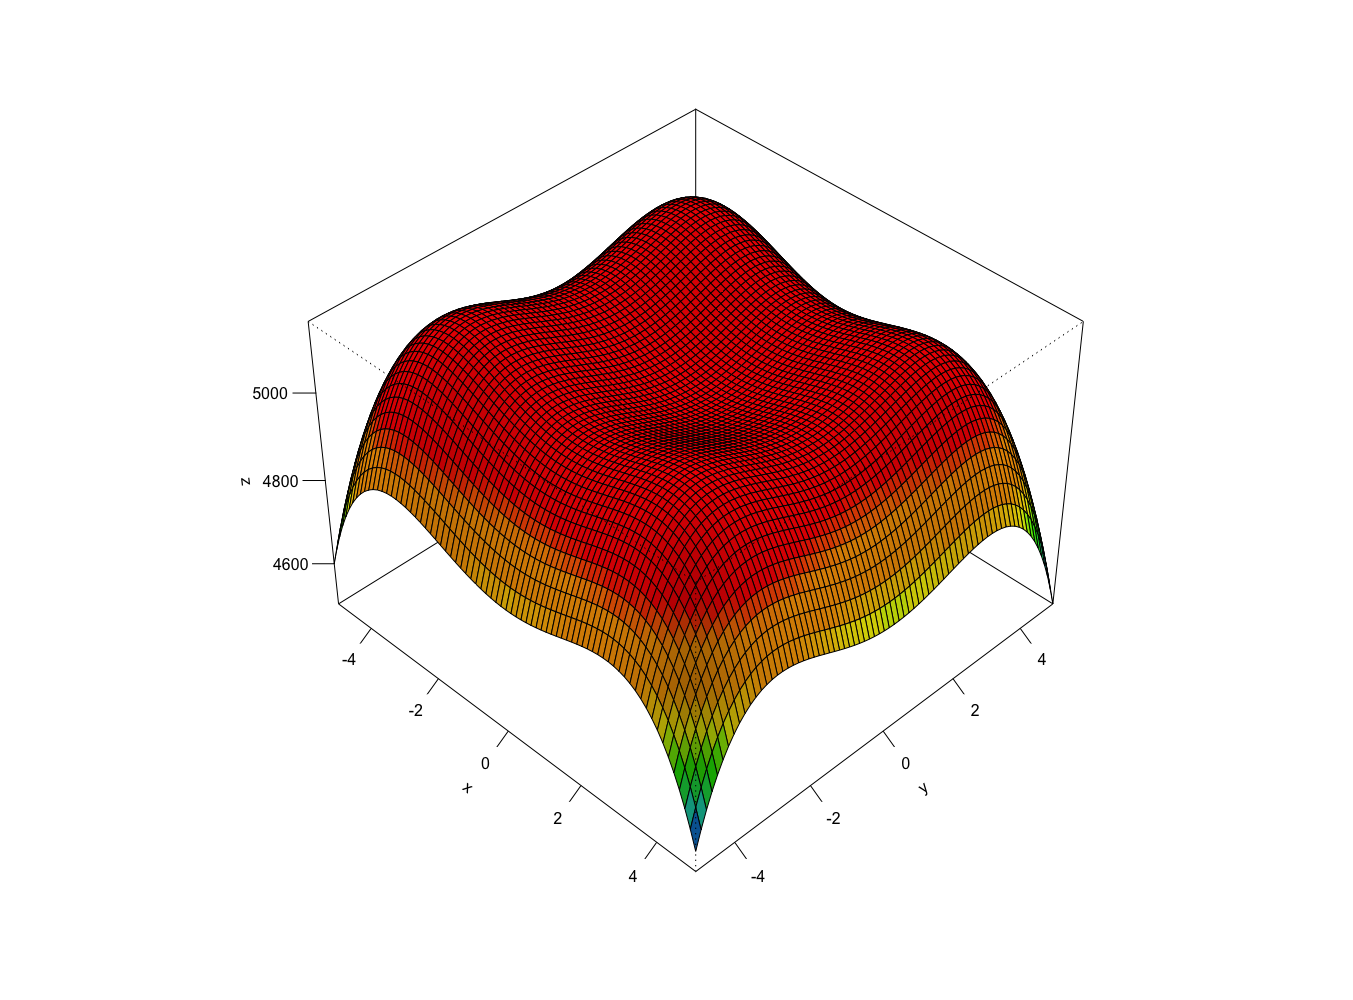
\includegraphics[width=1.7in]{customizedStyblinski}} \\
		\hline
	\end{tabular}
\end{sidewaystable}

\subsection{Algorithm' s Configuration} The RL algorithm employed is the {\tt SARSA($\lambda$)} one. It has only one configuration (summarized in table ~\ref{ConfigurationTable}) and four different declinations (summarized in table ~\ref{DeclinationTable}).

\begin{table} [h!]
	\centering
	\resizebox{\linewidth}{!} {	
	\begin{tabular}{|c||c|c|c|c|c|c|c|}
		\hline 
		& \textbf{$\lambda$}  & \textbf{$\epsilon$} & \textbf{qInit} & \textbf{Learning Rate} & \textbf{Discount Factor}  & \textbf{Episodes}  & \textbf{Epochs} \\
		\hline \hline Configuration $1$
		& $0.1$ & $0.1$ & $0$ & $1$ & $0.99$  & $150$ & $100$  \\ 
		\hline
	\end{tabular}
}
\caption{Configuration Table}
\label{ConfigurationTable}
\end{table}

\begin{table} [h!]
	\centering	
	\begin{tabular}{|c||c|}
		\hline \textbf{Declination}
		& \textbf{Type of search} \\ 
		\hline \hline Declination 1
		&  Linear, not random search\\ 
		\hline Declination 2
		& Linear, random search \\ 
		\hline Declination 3
		& Parametric, not random search \\ 
		\hline Declination 4
		&  Parametric, random search\\ 
		\hline 
	\end{tabular} 
\caption{Declination table}
\label{DeclinationTable}
\end{table}

In the proposed configuration a low $\lambda$ value is employed. Typically it should be used lower learning rate when a higher value of $\lambda$ is employed. However, in this case, it has been decided to use the highest possible learning rate. The logical consequence to this choice is to decrease the $\lambda$ value. \\

An $\epsilon$ value equals to $0.1$ means that $90\%$ of selected actions depends on the history, whereas the remaining $10\%$ represents a random choice having absolutely no relations with the previous history. \\ 

A discount factor set to $0.99$ means the rewards will propagate as long as possible through time.

The main goal presented in this work is to compare human optimization performances with {\tt SARSA($\lambda$)} ones in a context of uncertainty. Assuming that each try has an high cost, the number of possible tries must be as low as possible assuring, at the same time, a reasonable training space. In order to satisfy these requirements, the number of episodes is set to $150$. Each episode is composed by $100$ epochs. Note that in addition to the $150$ training episodes there is also a greedy one. In this last episode the $\epsilon$ value and the \textit{learning rate} parameter are set to $0$. Instead, the number of epochs, the {\tt qInit} parameter and the discount factor are left unchanged.  \\

Each declination of {\tt SARSA(\textit{$\lambda$})} corresponds to one combination of search techniques described in the previous chapter. In the implementation of random search, the BURLAP {\tt RandomFactory} class has been used. {\tt RandomFactory} allows to logically group various random generators. The {\tt id} is set to $0$ and the {\tt seed} is set to $1$.

\section{Experiment on Humans}

The test conducted on humans affects a cross-section of twenty-three people. In the selection process of test subjects the following three parameters with corresponding bounds were considered :

\begin{itemize}
	\item \textbf{Sex} $\in \{Male, Female\}$
	\item \textbf{Age} $\in [4, 52]$
	\item \textbf{Calculus Knowledge} $\in \{Null, Basic, Advanced\}$ 
\end{itemize}  

Each one of the test subjects was placed in front of a personal computer. The following rules have been proposed :

\begin{itemize}
	\item \textit{You will be offered four different levels}.
	\item \textit{The first three levels will need to be repeated three times}.
	\item \textit{The last level can be executed only once}.
	\item \textit{Look carefully at the legend before starting the experiment}.
	\item \textit{At each click you will receive a score with a colour associated with it}.
	\item \textit{The goal is to make as many points as possible with 15 clicks available for each game}.
	\item \textit{No further explanation will be provided}.
\end{itemize}

After that a chromatic scale indicating how positive the reward was for each click was proposed.

\begin{figure}[h!]
	\centering
	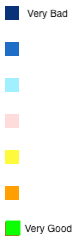
\includegraphics{scala.png}
	\caption{Chromatic Scale.}
	\label{fig:Cromatic Scale}
\end{figure}

A white screen (with a specific hidden function) of $600 \times 600$ pixels with which to interact according to the rules previously listed was finally proposed. \\







